\documentclass{article}
\usepackage{graphicx} % Required for inserting images
\usepackage{animate}
\usepackage{subcaption}
\usepackage{booktabs}
\usepackage[utf8]{inputenc}
\usepackage[french]{babel}
\usepackage[T1]{fontenc}
\usepackage[a4paper,top=1cm,bottom=1.2cm,left=1cm,right=1cm,marginparwidth=1.75cm]{geometry}

\usepackage{chngcntr} 
\usepackage{comment}
\usepackage{amsmath}
\usepackage{physics}
\usepackage{xurl}
\usepackage{soul,xcolor}
\usepackage{siunitx}
\usepackage[backend=biber, style=numeric, sorting=none]{biblatex}

\addbibresource{references.bib}
\usepackage{float}
\usepackage[colorlink = true]{hyperref}
\setulcolor{violet}
\title{Projet expérimental :\\
Observation du caractère chaotique du circuit de Chua}
\author{Adam Franchot--Fowler \\Corentin Duclos\\Groupe C-01}
\date{}

\begin{document}

\maketitle
\tableofcontents
\section{Introduction}
En 1983, Leon Chua \cite{chua2007chua} conçoit le circuit qui porte désormais son nom pour lever deux verrous scientifiques majeurs liés aux équations de Lorenz. \\

Le premier consistait à réaliser un système physique concret, constructible en laboratoire et fidèlement modélisable par ces équations, afin de démontrer expérimentalement que le chaos est un phénomène physique intrinsèque et non un artefact numérique engendré par les erreurs d'arrondi des simulations informatiques.\\ Le second visait à établir, par une démonstration mathématique rigoureuse, que l'attracteur de Lorenz jusqu'alors uniquement observé par voie numérique possédait bien les propriétés chaotiques théoriques attendues.\\

L'entreprise se révéla fructueuse : l'existence d'attracteurs chaotiques au sein du circuit de Chua fut d'abord confirmée par les simulations numériques de Matsumoto en 1984, puis observée expérimentalement par Zhong et Ayrom en 1985.\\

Au-delà de l'attracteur chaotique dit « double-scroll » sa signature la plus emblématique, le circuit de Chua s'est révélé d'une remarquable richesse dynamique, engendrant une grande variété de comportements attractifs selon les valeurs des paramètres de contrôle. On distingue notamment les points fixes, correspondant à un régime stationnaire stable ; les cycles limites, associés à une oscillation périodique ; les attracteurs quasi-périodiques (attracteur de Rössler) et « double-scroll », présentant une sensibilité exponentielle aux conditions initiales et une structure fractale.\\

Fort de cet ancrage historique, nous nous proposons dans ce projet expérimental de créer le circuit de Chua et d'étudier la transition vers le chaos en observant et en analysant la cascade de doublement de période, obtenue par la variation contrôlée des paramètres du système.

\clearpage
\section{Partie théorique}

\subsection{Circuit de Chua}
\subsubsection{Généralités}
Dans le cadre de cette étude nous allons considérer un circuit de Chua dans une configuration standard \cite{hobson1996simple}. Ainsi notre circuit sera composé de deux condensateurs, d'une bobine, d'une résistance linéaire, et d'un élément non linéaire appelé diode de Chua. Le tout sera monté sous la forme suivante :
\begin{figure}[H]
\centering
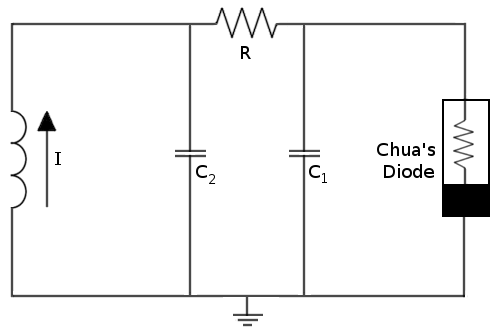
\includegraphics[width=0.4\textwidth]{Chuacircuit's.png}
\caption{Circuit de Chua}
\end{figure}
La diode de Chua jouera le rôle d'une résistance négative non linéaire. Aussi on note 
\begin{itemize}
    \item $v_1$ la tension aux bornes de $C_1$,
    \item $v_2$ la tension aux bornes de $C_2$,
    \item $i_L$ l'intensité dans la bobine $L$.
\end{itemize}
En utilisant les lois de Kirchhoff on peut obtenir le système d'équations suivant
\begin{align}
C_1 \dv{v_1}{t} &= \frac{v_2-v_1}{R} - g(v_1), \\
C_2 \dv{v_2}{t} &= \frac{v_1-v_2}{R} + i_L, \\
L \dv{i_L}{t} &= -v_2.
\end{align}
Où la fonction $g$ décrit la caractéristique tension-courant non linéaire de la diode de Chua, que l'on décrira plus en détail par la suite.\\
Les régimes dynamiques du circuit s'obtiennent en étudiant les points fixes du système, c'est-à-dire les états pour lesquels
\[
\dv{v_1}{t}=\dv{v_2}{t}=\dv{i_L}{t}=0.
\]
Selon les valeurs des paramètres, ces points fixes peuvent être stables ou instables. Lorsqu'un point fixe perd sa stabilité, le système peut bifurquer vers un régime périodique, puis vers des oscillations plus complexes, parfois chaotiques.\\
On distingue alors :
\begin{itemize}
    \item \textbf{Points fixes :} le système atteint un état stationnaire.
    \item \textbf{Oscillations périodiques :} les variables évoluent de façon répétitive avec une période bien définie.
    \item \textbf{Chaos déterministe :} le système reste régi par des équations déterministes, mais son évolution devient non périodique et très sensible aux conditions initiales.
\end{itemize}
Ceci peut être résumé dans un diagramme de bifurcation classique comme celui-ci, où l'abscisse représente un des paramètres de contôle du circuit et le nombre de points à une abscisse donnée représente le nombre de périodes avant de retourner à l'état initial (la partie de gauche correspond donc à une période, celle du milieu à deux périodes, celle de droite à plus de deux périodes ou du chaos):
\begin{figure}[H]
\centering
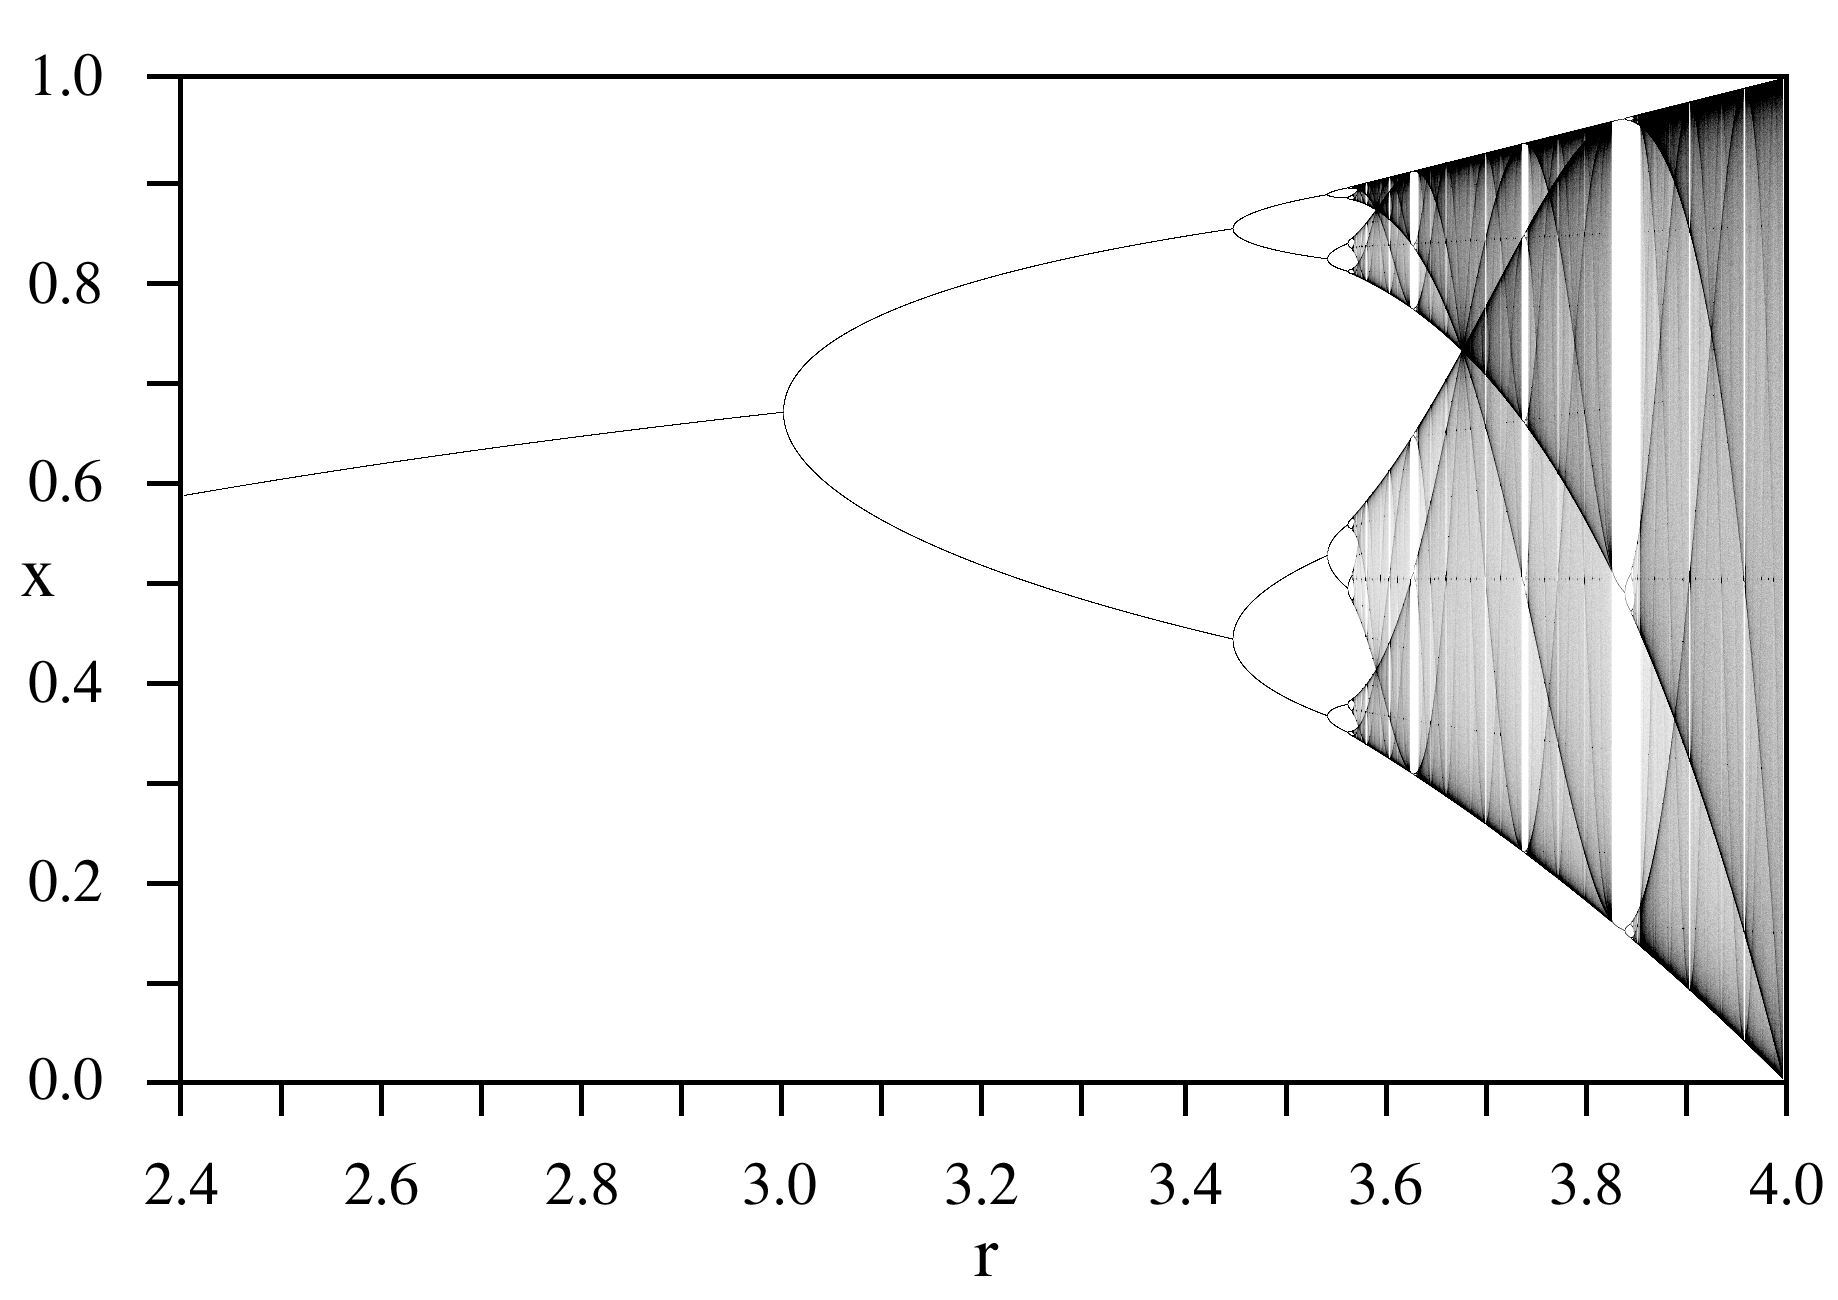
\includegraphics[width=0.3\textwidth]{BifurcationDiagram.png}
\caption{Diagramme de bifurcation}
\end{figure}
\subsubsection{Pourquoi la Diode de Chua?}
La présence d'un composant non linéaire est ici indispensable. En effet, un circuit purement linéaire ne peut produire que des régimes transitoires amortis ou des oscillations sinusoïdales entretenues~: son comportement est entièrement déterminé par les valeurs propres de
sa matrice d'évolution, et aucune dynamique complexe n'est possible. La non-linéarité introduite par la diode de Chua brise cette contrainte~: elle permet au système de quitter un point fixe instable sans diverger pour autant, et c'est précisément cette tension entre instabilité locale et confinement global qui est à l'origine des comportements chaotiques observés. De plus, il ne suffit pas d'introduire n'importe quelle non-linéarité~: il est nécessaire que le composant présente une résistance négative sur une plage de tension. Une résistance positive dissipe de l'énergie, ce qui tend à amortir toute oscillation. À l'inverse, une résistance négative compense ces pertes en injectant de l'énergie dans le circuit, empêchant ainsi le système de converger vers un point fixe stable. C'est cette alimentation locale en énergie, couplée au confinement assuré par les parties à résistance positive aux extrémités de la caractéristique, qui permet au circuit d'entretenir des oscillations sans pour autant diverger. Sans cette propriété, le circuit de Chua ne serait qu'un simple oscillateur amorti, incapable de générer l'attracteur qui fait toute sa richesse.

\subsubsection{Zoom sur la diode de chua}

Dans le cadre de ce projet expérimental nous construirons la diode de Chua sous la forme suivante \cite{kennedy1992robust} :
\begin{figure}[H]
\centering
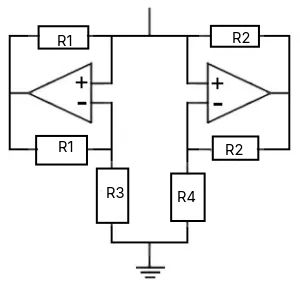
\includegraphics[width=0.3\textwidth]{diode chua.png}
\caption{Diode de Chua}
\end{figure}
On va commencer à chercher l'expression explicite de g, à savoir la fonction de la caractéristique tension courant de la diode. Pour cela nous commencerons par faire l’hypothèse que les amplificateurs sont en régime linéaire où $v_s=v_+-v_-$. Avec cette dernière info on peux obtenir explicitement g sous la forme :
\begin{equation}
    g(V) = G_bV+\frac{1}{2}(G_a-G_b)(|V+E|-|V-E|).
\end{equation}
Où les différentes inconnues sont :
\begin{align}
    &G_a = -\frac{1}{R_3}-\frac{1}{R_4} \\
    &G_b= -\frac{1}{R_4}+\frac{1}{R_1} \\
    &E=\frac{R_3}{R_3+R_1}E_{sat}
\end{align}

Avec $E_{sat}$ la tension de saturation des amplificateurs utilisés. Cela donne une courbe tension-courant de la forme :

\begin{figure}[H]
\centering
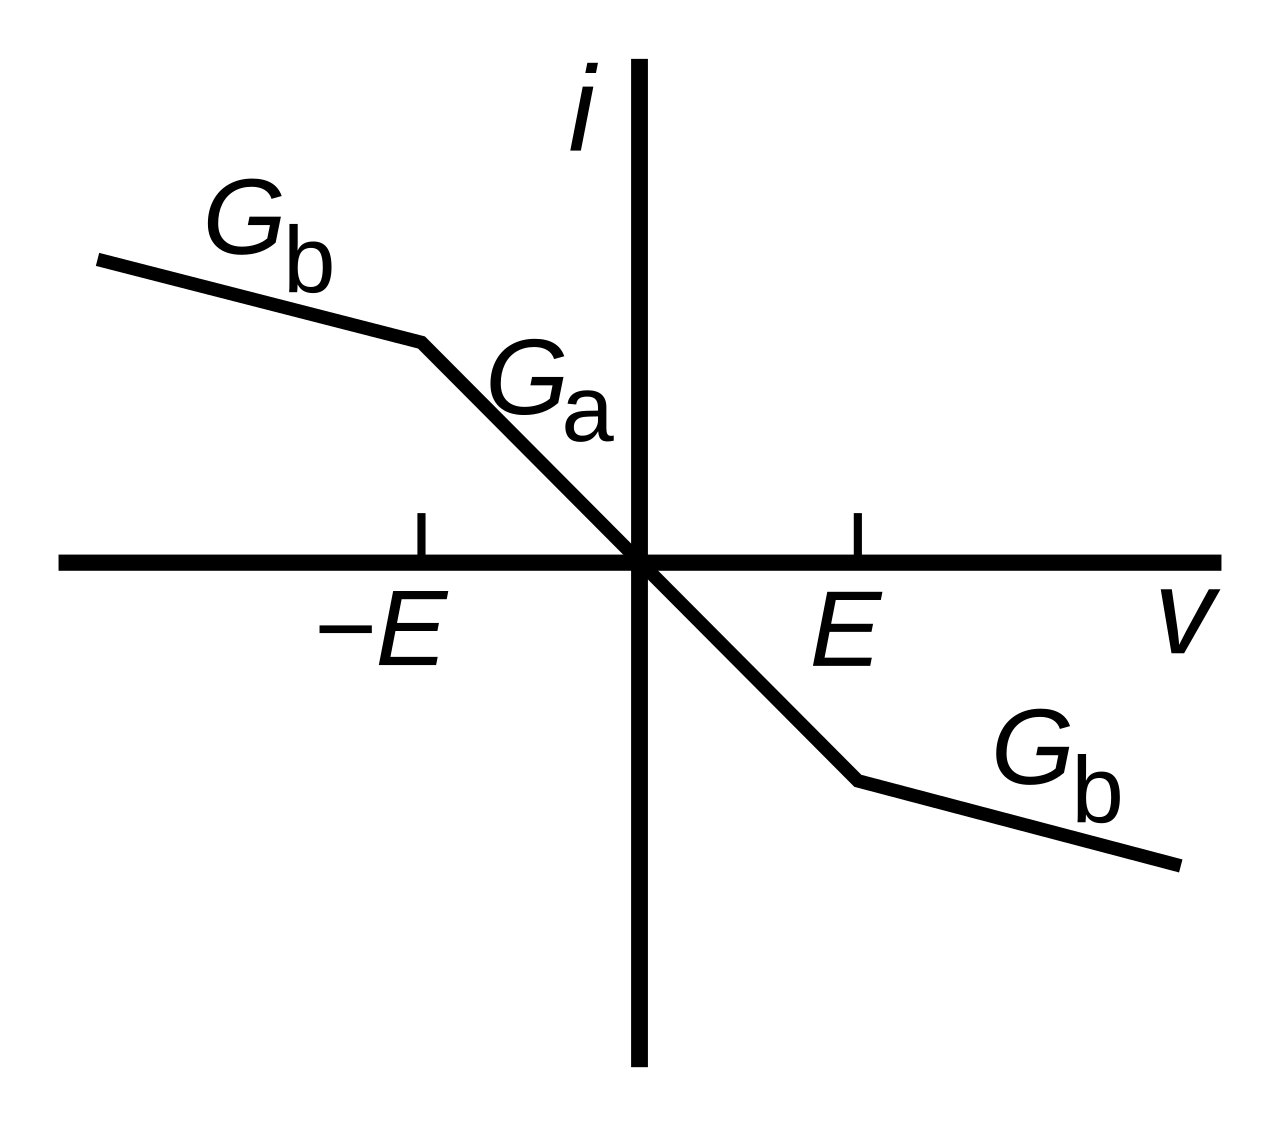
\includegraphics[width=0.3\textwidth]{courbe fonctionnement diode.png}
\caption{Courbe tension-courant de la diode de Chua}
\end{figure}

\subsection{Constante de Feigenbaum}
Dans le cadre de l'étude des transitions vers le chaos dans les systèmes non linéaires, Feigenbaum a mis en évidence, à la fin des années 1970, une propriété remarquable et universelle associée aux cascades de dédoublement de période \cite{strogatz2018nonlinear}. Lorsqu'un paramètre de contrôle du circuit --- ici typiquement la résistance $R$ --- est progressivement varié, le système ne bascule pas brutalement dans le chaos~: il y transite de manière ordonnée, en passant successivement par des régimes périodiques de période $T$, puis $2T$, $4T$, $8T$, et ainsi de suite. Chacun de ces dédoublements correspond à une bifurcation de type fourche, et leur accumulation constitue ce que l'on appelle une \textbf{cascade de period-doubling}.

On note $R_1, R_2, R_3, \dots$ les valeurs du paramètre auxquelles apparaissent ces bifurcations successives. La vitesse à laquelle elles s'accumulent est capturée par la suite de rapports~:
\begin{equation}
    \delta_n = \frac{R_{n+1} - R_n}{R_{n+2} - R_{n+1}}
\end{equation}
qui mesure le facteur de compression entre deux intervalles consécutifs. Feigenbaum a montré que, quelle que soit la forme précise de la non-linéarité du système, cette suite converge vers une constante universelle~:
\begin{equation}
    \delta = \lim_{n \to \infty} \delta_n \approx 4{,}669
\end{equation}
Cette constante, désormais appelée \textbf{constante de Feigenbaum}, signifie concrètement que chaque intervalle de bifurcation est environ 4{,}669 fois plus étroit que le précédent~: les dédoublements s'accélèrent et s'accumulent en un point fini $R_\infty$, au-delà duquel le comportement chaotique s'installe.

L'universalité de $\delta$ est particulièrement frappante~: elle s'applique à une très large classe de systèmes dynamiques, des applications unimodales aux circuits électroniques non linéaires, dont le circuit de Chua fait partie.
\section{Partie Expérimentale}

\subsection{Diode de Chua}

Nous avons donc réalisé le montage de la diode de Chua comme prévu par la partie théorique, avec des valeurs de résistances R1=220 $\Omega$, R2=22 $k\Omega$, R3=2,2 $k\Omega$, R4=3,3 $k\Omega$ et des amplificateurs avec 15V de tension de saturation \cite{kennedy1992robust} (toutes ces valeurs ont des incertitudes à $\pm5\%$ selon les constructeurs) :

\begin{figure}[H]
\centering
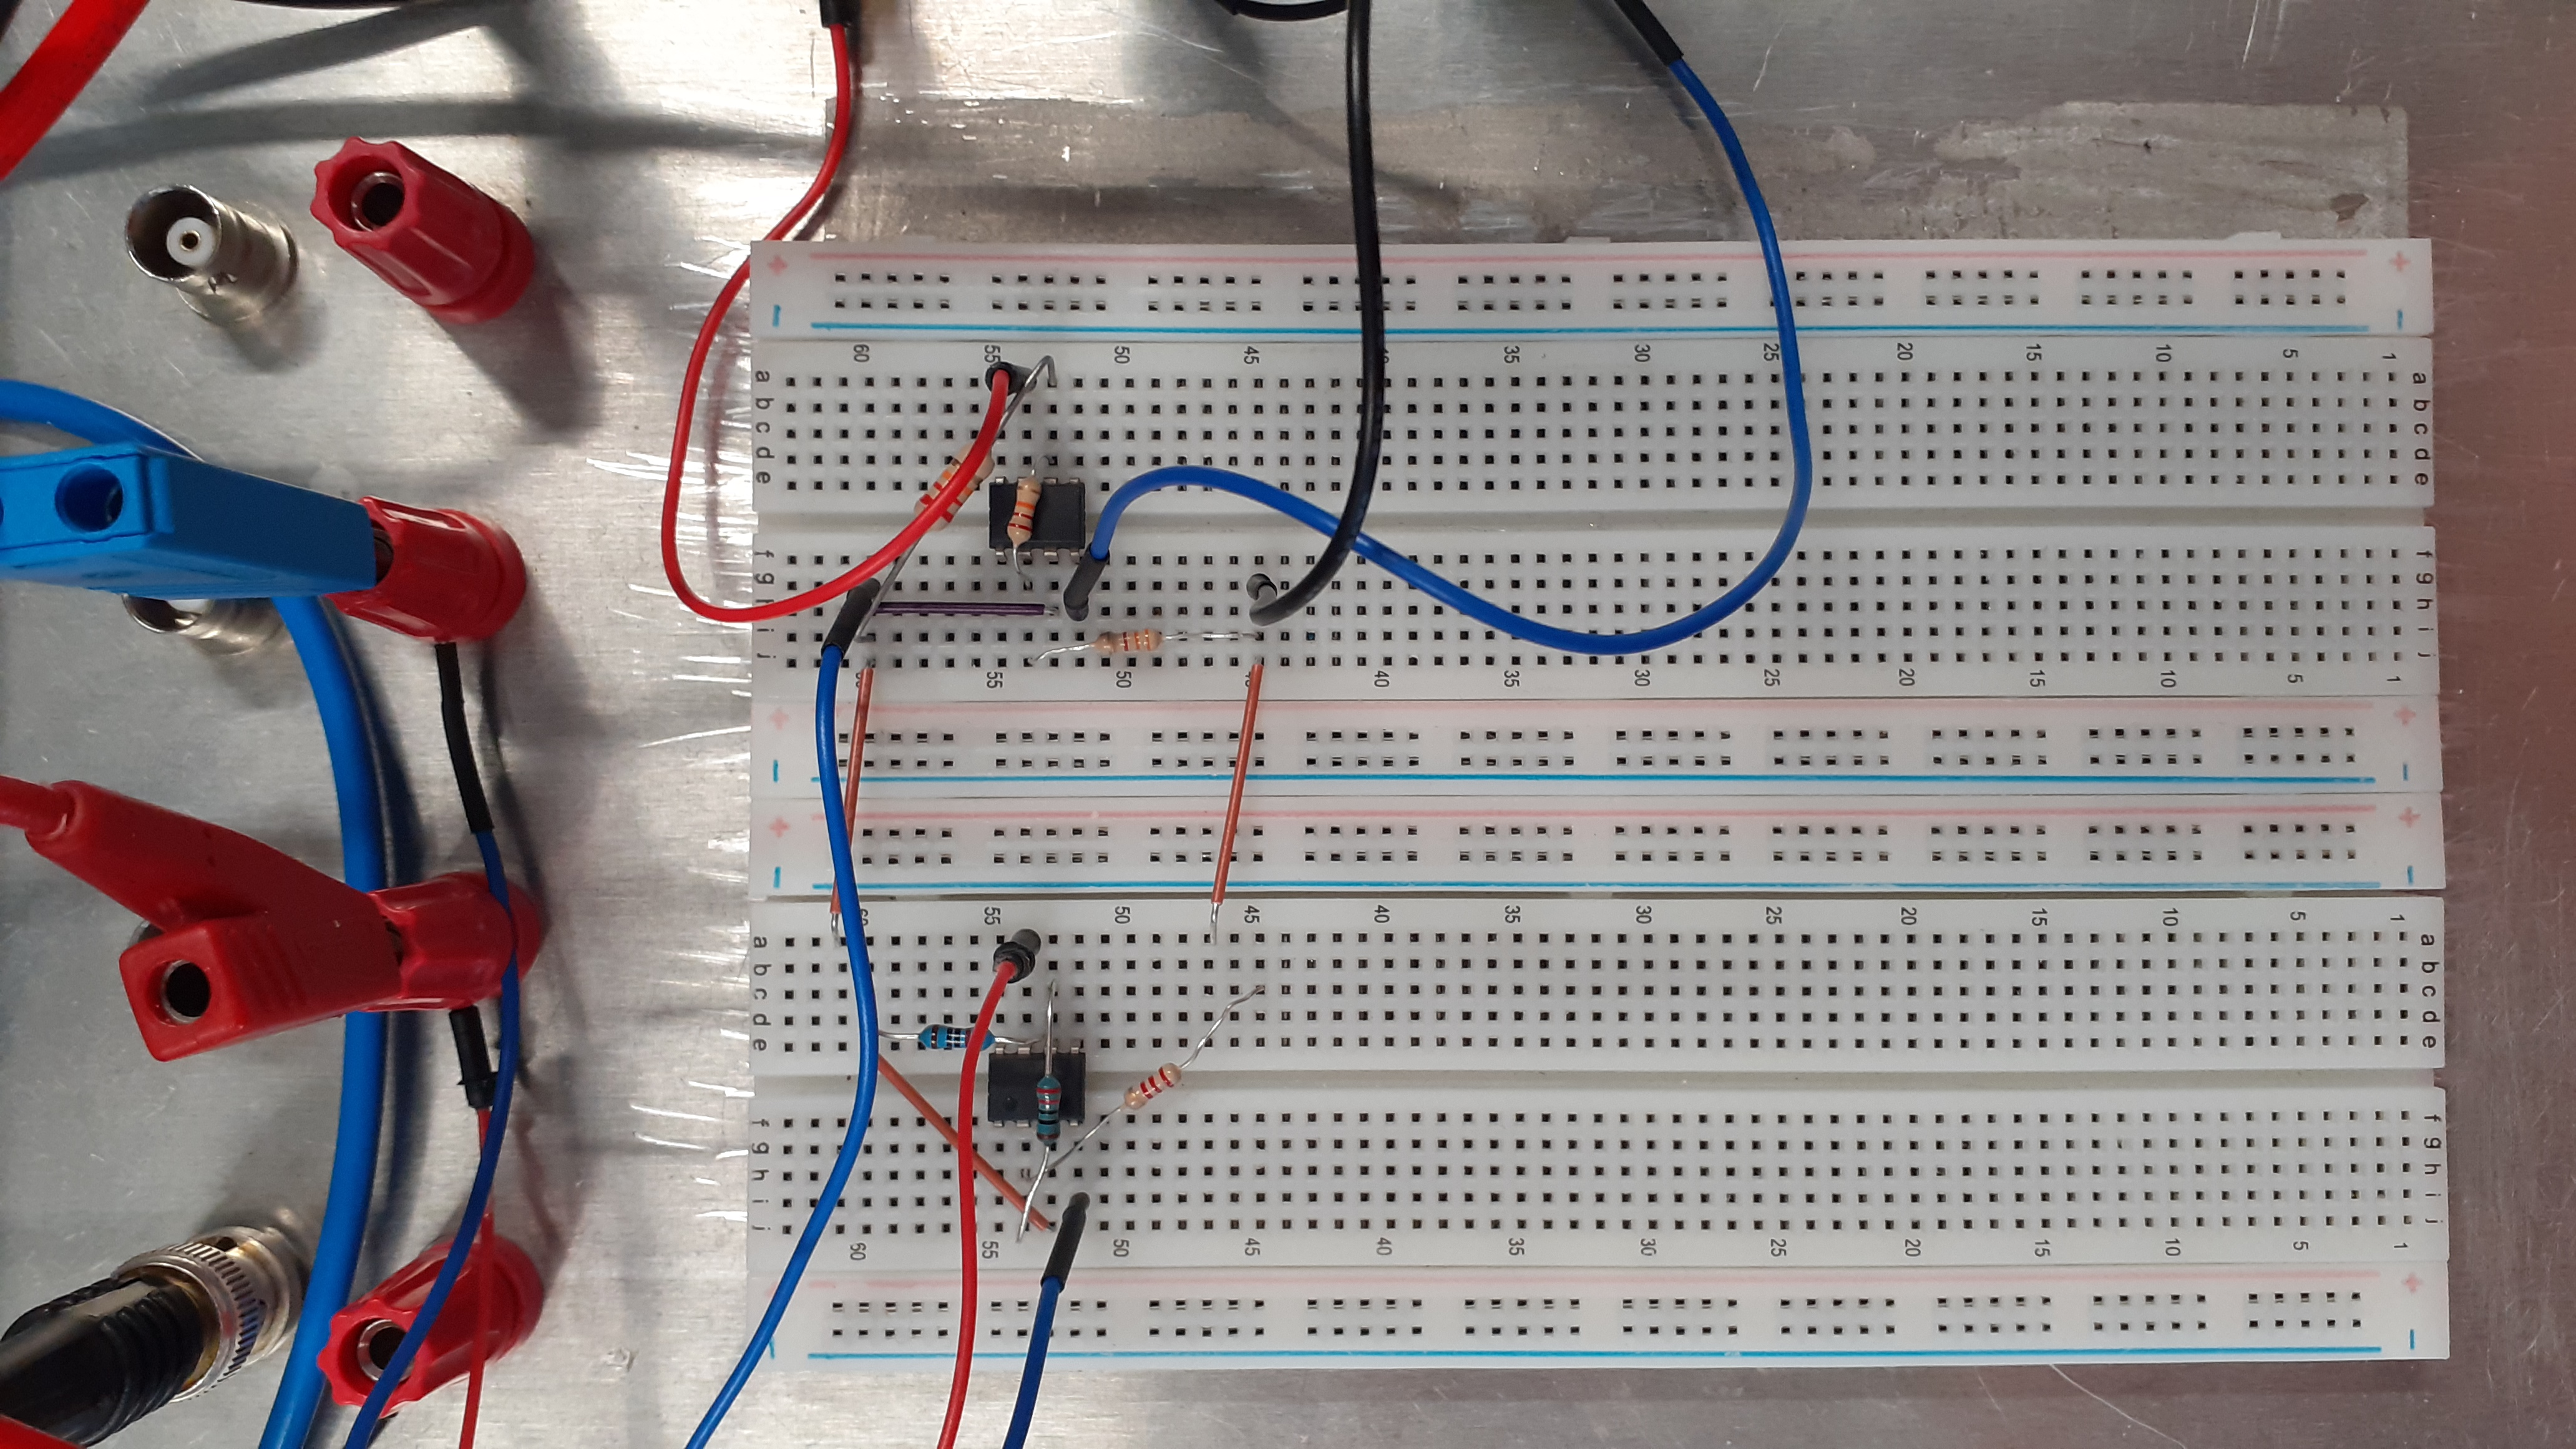
\includegraphics[width=0.5\textwidth]{image montage diode.jpg}
\caption{Montage de la diode de Chua}
\end{figure}

Afin de vérifier que la diode fonctionne, il faut tracer sa courbe intensité-potentiel et vérifier que l'on obtient les ruptures de pentes aux bonnes valeurs de tension. Afin de tracer cette courbe, nous utilisons une carte sysam-sp5 pour acquérir les données et traçer des courbes et un oscilloscope pour voir en direct ce qu'il se passe dans le circuit. Ces deux appareils ne pouvant mesurer que des tensions pas de courant, on a placé une résistance en série de la diode de Chua et mesuré sa tension, nous donnant accès à l'intensité dans le circuit. Enfin, nous plaçons un générateur de tension alternative pour voir l'intensité pour toutes les valeurs de potentiel. Cela nous donne donc la courbe suivante :

\begin{figure}[H]
\centering
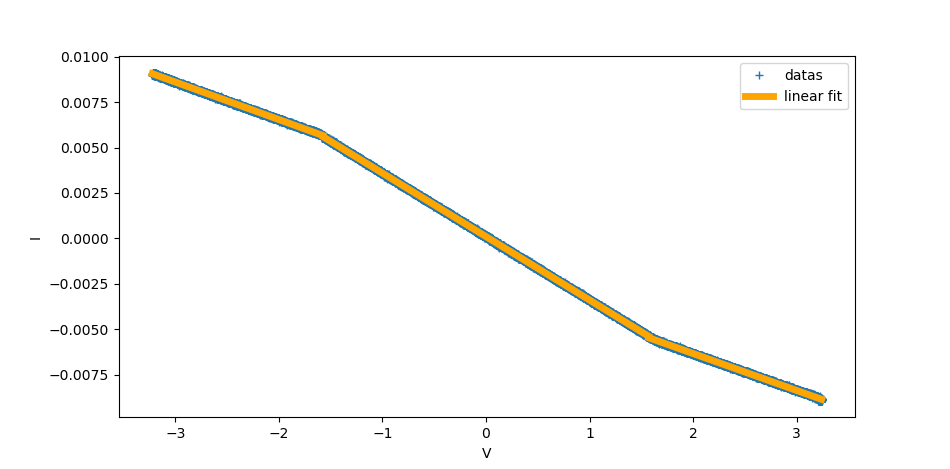
\includegraphics[width=0.5\textwidth]{IVdiodedechuapng.png}
\caption{Courbe intensité-potentiel de la diode de Chua (l'intensité est amplifiée fois 5)}
\end{figure}

A l'aide d'une régression linéaire nous avons obtenu les valeurs des pentes : $(-4,1\pm0,2)*10^{-4}\Omega^{-1}$ à gauche, $ (-7,0\pm0,3)*10^{-4}\Omega^{-1} $ au milieu et $(-4.1\pm0,2)*10^{-4}\Omega^{-1}$ à droite. Avec les formules de la partie théorique et les valeurs de résistances utilisées, on a théoriquement des pentes de $(-4,1\pm0,3)*10^{-4}\Omega^{-1}$ sur les bords et $(-7,6\pm0,6)*10^{-4}\Omega^{-1}$ au centre. L'expérimental est donc en accord avec la théorie pour les pentes.\\

Et nous pouvons retrouver les abscisses des coudes : $(-1,6\pm0,2) V$ à gauche et $(1,4\pm0,2) V$ à droite. La valeur théorique avec les résistances et amplificateurs est de $(\pm1,9\pm0,3)V$.
Ces valeurs ne sont pas complètement en accord, les coudes tombent tout juste en dehors de leurs incertitudes respectives. Les valeurs sont cependant similaires.\\

Nous avons donc réalisé une diode de Chua qui est fonctionnelle et presque en accord avec la théorie.

\subsection{Circuit de Chua}

A l'aide de cette diode de Chua nous pouvons donc maintenant réaliser le circuit de Chua. Pour cela, on utilise une résistance et une inductance variables afin de pouvoir modifier les paramètres du circuit. On place aussi une résistance en série de la bobine pour avoir accès à $i_L$. Cette résistance est faible, du même ordre de grandeur que la résistance interne de la bobine (une dizaine d'Ohms) afin de ne pas trop influencer le circuit. Elle est cependant faible pour nos mesures aussi et nous avons dû l'amplifier 100 fois pour l'obtenir en détail. Cela nous donne le montage suivant :

\begin{figure}[H]
\centering
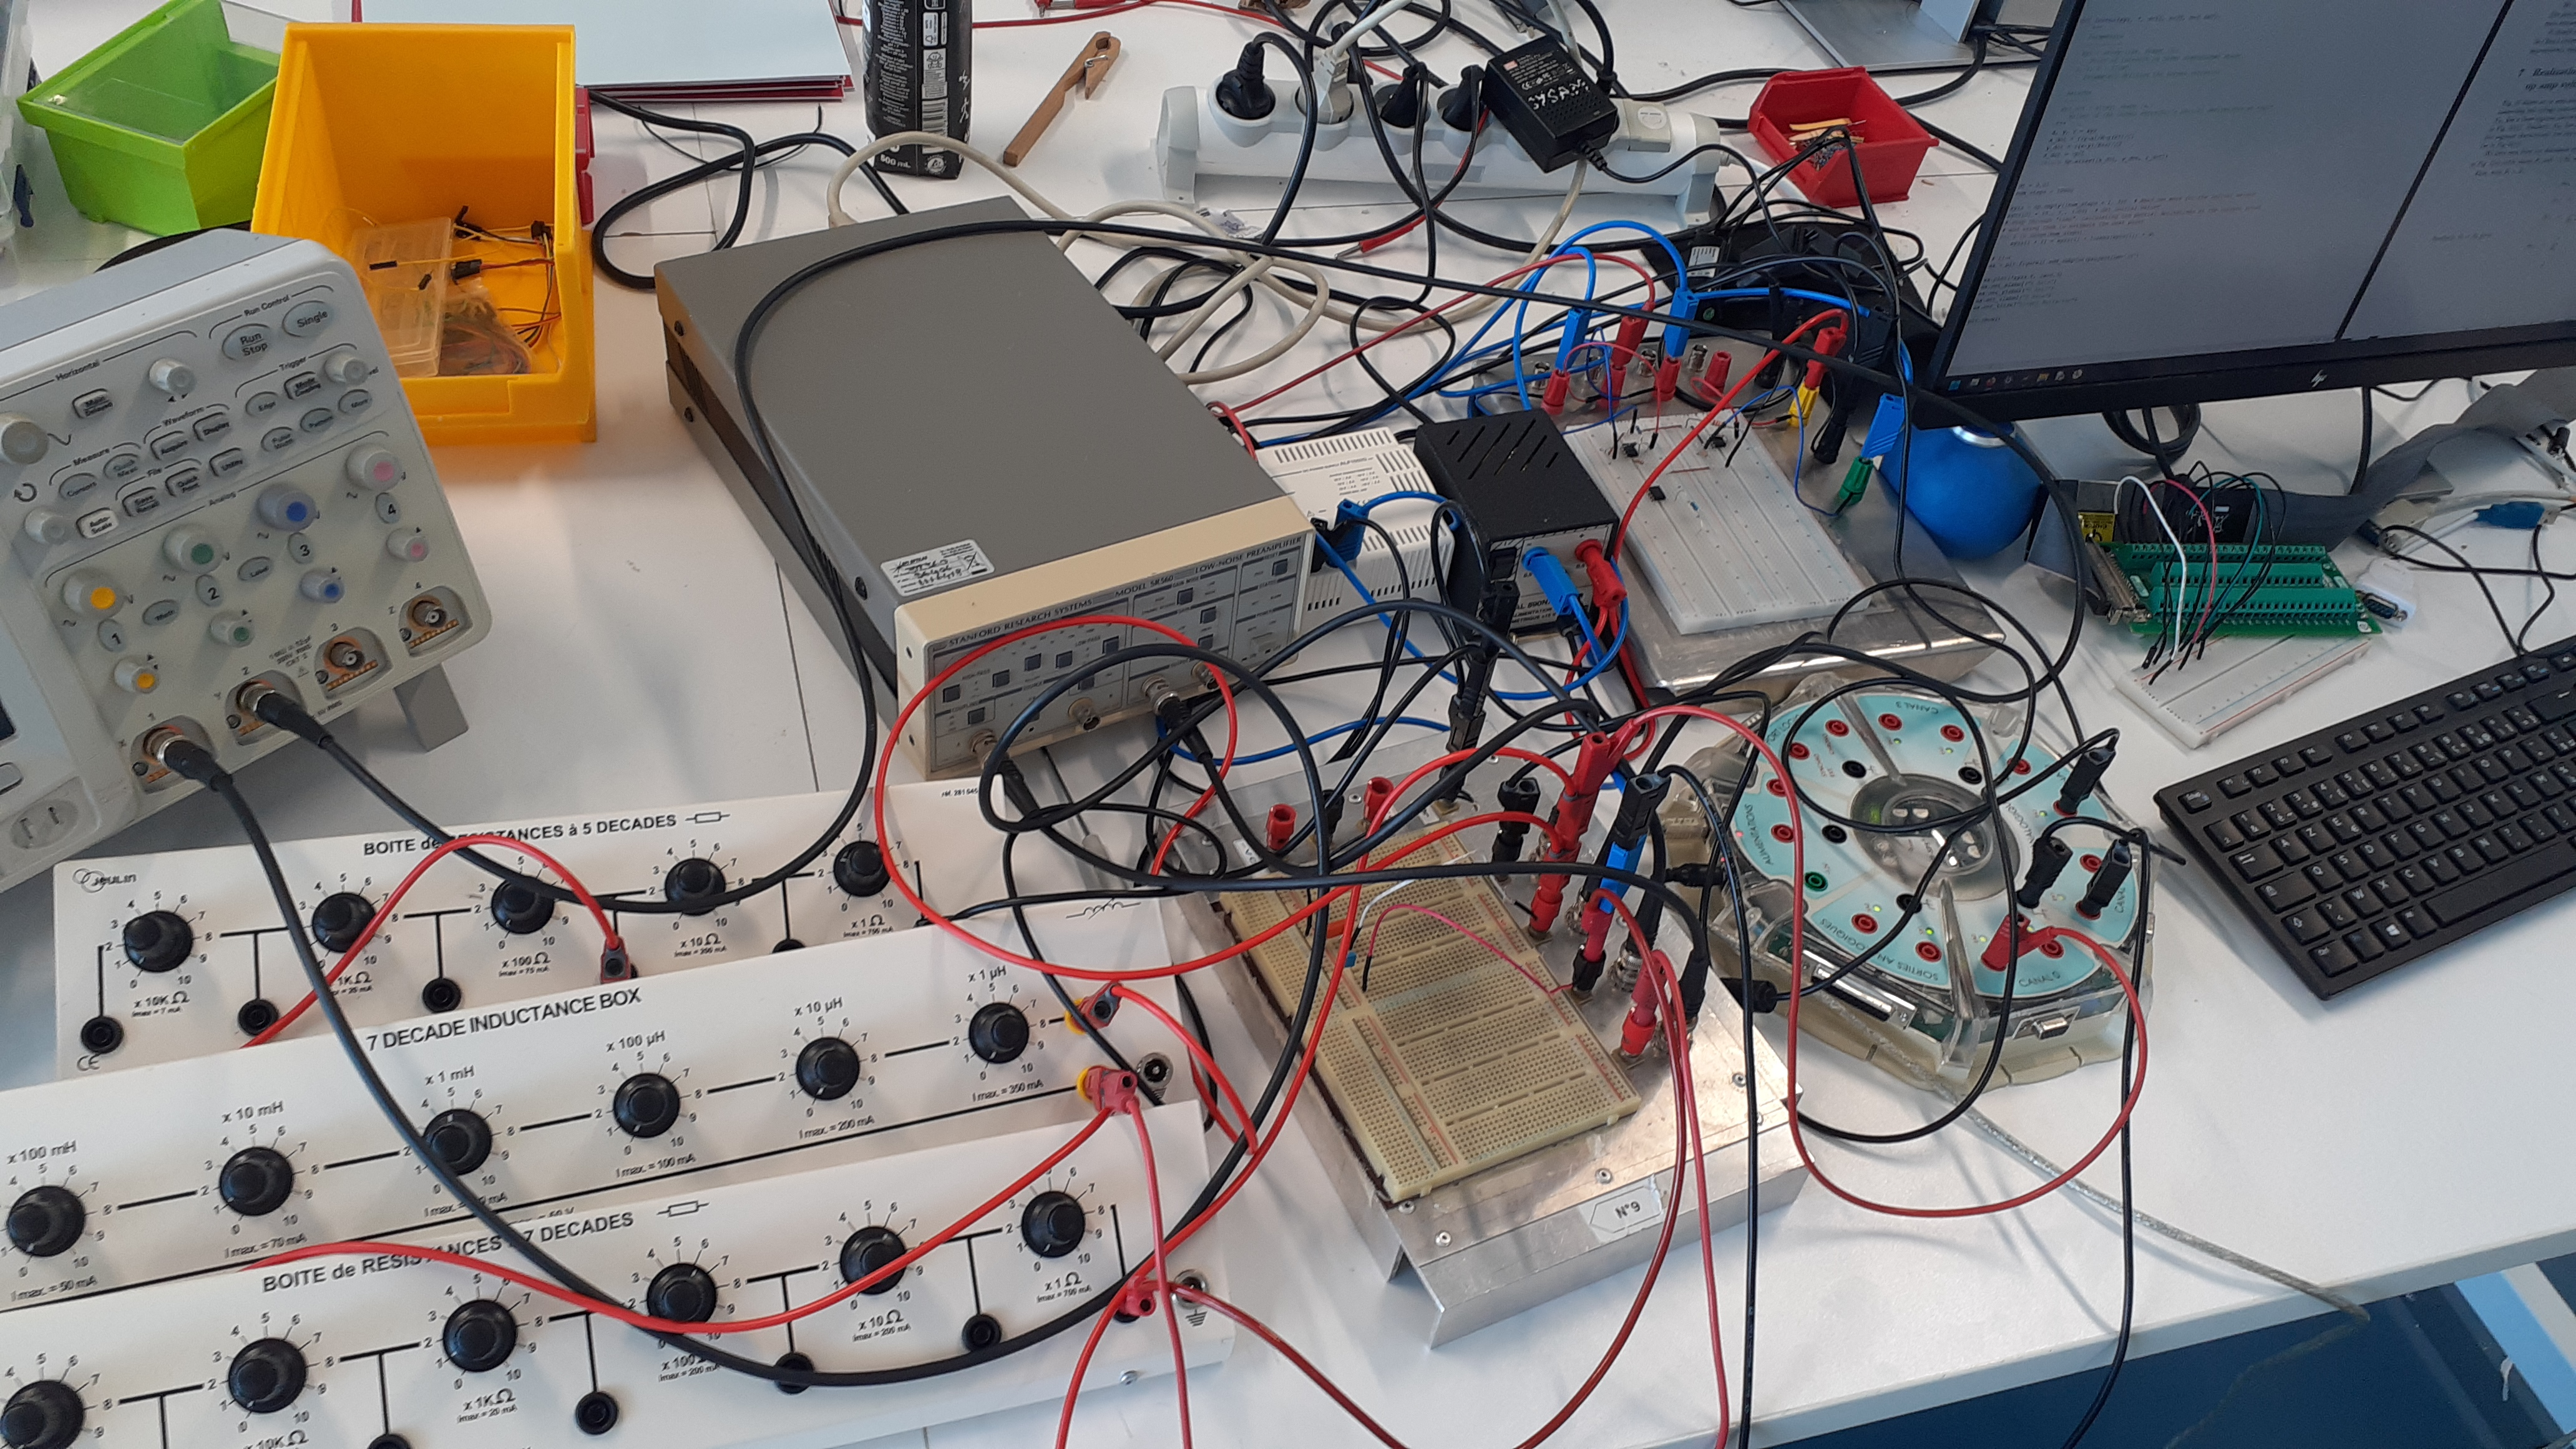
\includegraphics[width=0.5\textwidth]{image montage circuit.jpg}
\caption{Montage du circuit de Chua}
\end{figure}

En faisant varier la résistance R à L=15mH fixé, on parvient à trouver le <<double-scroll>>, ce qui nous indique que le circuit de Chua réalisé est fonctionnel et permet bien d'observer le chaos :

\begin{figure}[H]
\centering
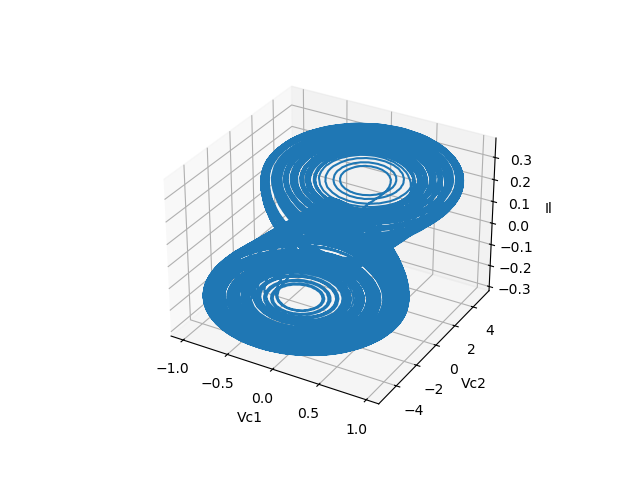
\includegraphics[width=0.4\textwidth]{image/chaos.png}
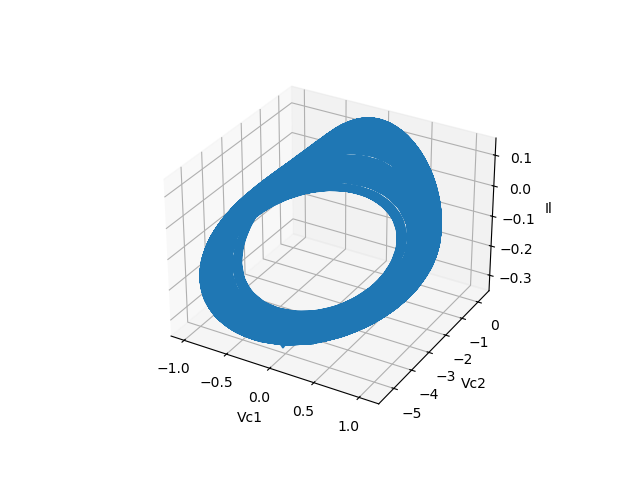
\includegraphics[width=0.4\textwidth]{image/surface_gauche.png}
\caption{Chaos : "Double-Scroll" et simple "Scroll"}
\end{figure}

Remarque : Pour obtenir des figures plus belles, le bruit a été enlevé lors des affichages par un lissage des valeurs brutes.\\
\\


On peut aussi chercher les autres régimes du système, comme les régimes périodiques :

\begin{figure}[H]
\centering
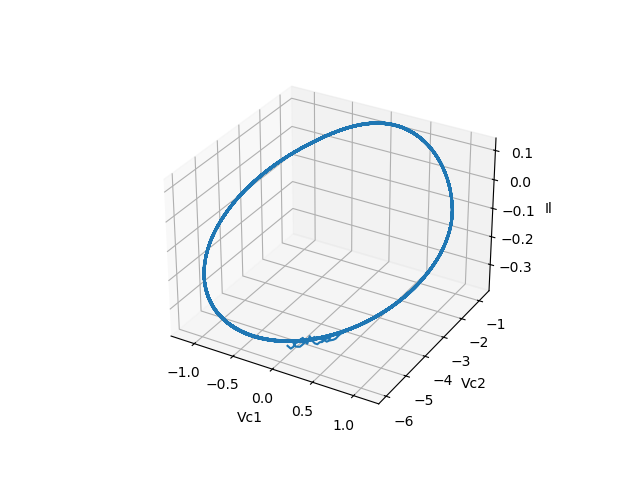
\includegraphics[width=0.4\textwidth]{image/1TG.png}
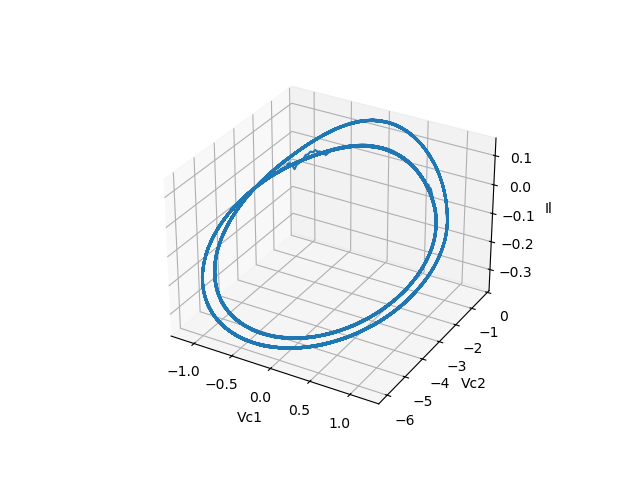
\includegraphics[width=0.4\textwidth]{image/2TG.png}
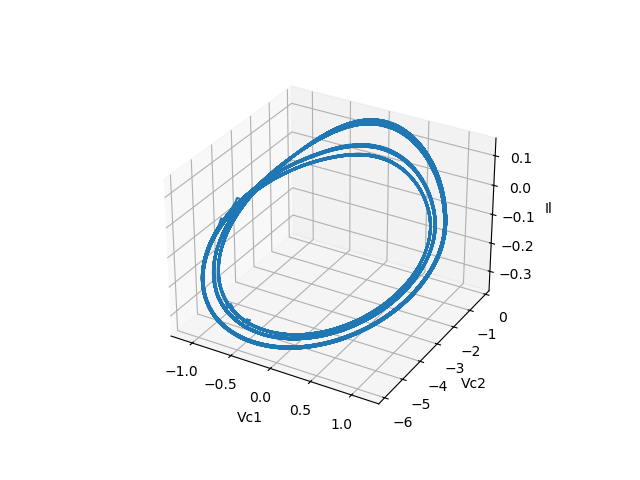
\includegraphics[width=0.4\textwidth]{image/4TG.png}
\caption{Différents régimes périodiques du système : 1, 2 et 4 périodes}
\end{figure}

Remarque : sur les figures périodiques et sur certains régimes chaotiques, on se situe sur l'un des deux côtés du "double-scroll", ces régimes peuvent être chaotiques car ils ne repassent jamais par les conditions initiales. Le "double-scroll" est un cas où le système passe aléatoirement de l'un à l'autre, il s'obtient en continuant à faire varier la résistance après avoir atteint le chaos en simple "scroll".\\

Les régimes périodiques sont de périodes en puissance de deux comme le montre le diagramme de bifurcation, et finit par arriver sur la situation chaotique. On remarque cependant dans le diagramme de bifurcation des zones au sein de la partie chaotique qui ne le sont pas : il y a des zones "blanches" où le nombre de périodes reste fini. C'est par exemple le cas sur le diagramme en r=3.85, où on remarque trois valeurs possibles. En cherchant un peu au sein du chaos nous avons réussi à trouver cette situation :

\begin{figure}[H]
\centering
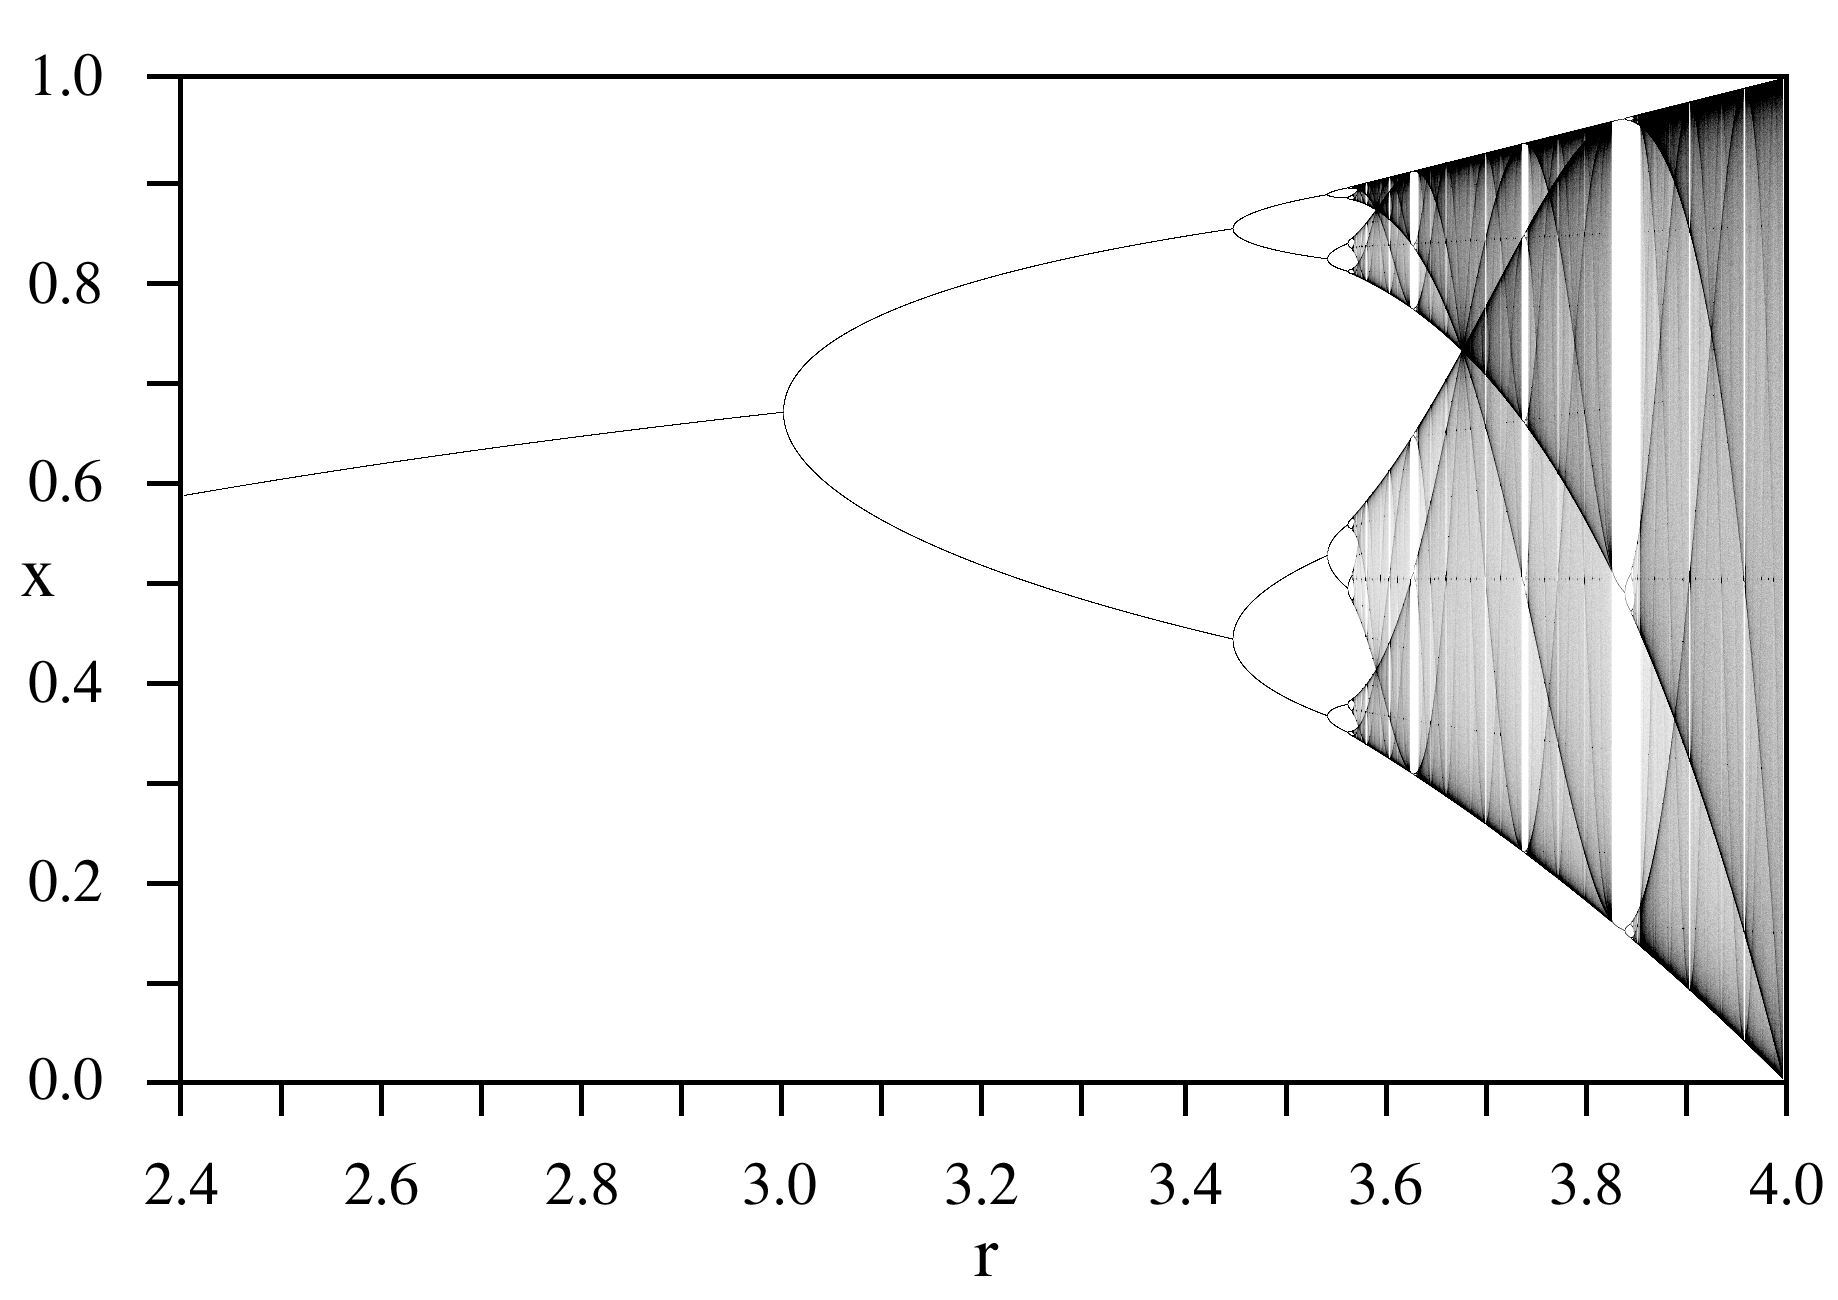
\includegraphics[width=0.4\textwidth]{BifurcationDiagram.png}
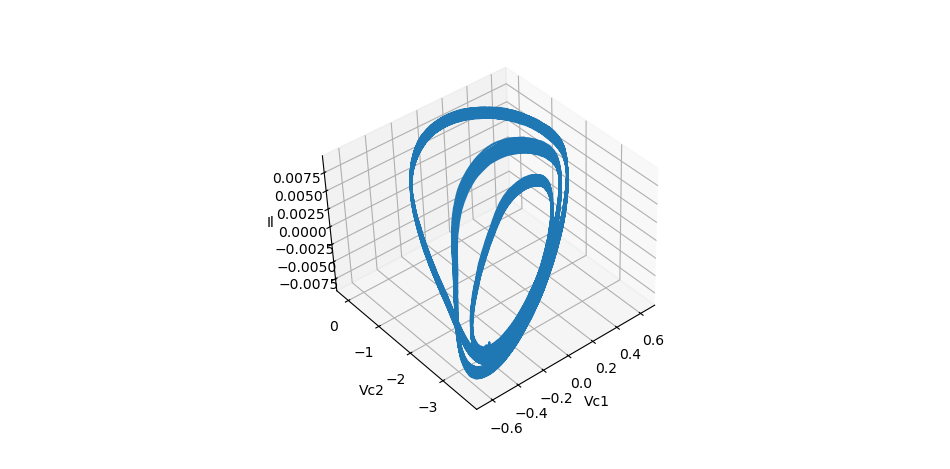
\includegraphics[width=0.8\textwidth]{image/3T.png}
\caption{Diagramme de bifurcation et régime à trois périodes}
\end{figure}

\subsection{Constante de Feigenbaum}

Nous souhaitons maintenant étudier la transition vers le chaos dans notre circuit de Chua. Pour cela, nous allons trouver grâce à notre montage les premières valeurs de la suite convergeant vers la constante de Feigenbaum.\\


Nous continuons avec le même protocole que précédemment : nous faisons varier la résistance variable à inductance fixée. Cependant maintenant nous mesurons expérimentalement la valeur de résistance lors des transitions entre les différents régimes de périodes en puissance de deux avant le chaos.\\

On ne peut cependant pas observer autant de transitions entre régimes que l'on souhaite car le système est un peu bruité, ce qui fait que différentier le cas de huit périodes de seize est compliqué (peu précis) et celui de seize périodes du chaos est impossible. En plus de cela, les transitions sont de plus en plus proches, elles finissent par être de l'ordre de grandeur de nos variations les plus fines vers seize périodes : On ne peut pas aller plus loin.\\

Dans notre cas, nous fixons l'inductance variable puis nous utilisons la résistance variable comme paramètre comme décrit précédemment. L'avantage d'avoir une inductance variable est qu'après avoir pris une série de valeurs de la résistance, nous pouvons modifier la valeur de l'inductance et recommencer, ce qui nous permet d'avoir plusieurs séries de données, et ainsi nous pouvons faire une moyenne, augmentant la précision de nos résultats.\\

Nous avons réalisé 7 séries de mesures (l'inductance variable utilisée ne nous permettait pas d'en faire plus car certaines des bobines étaient cassées) :

\begin{figure}[H]
\centering
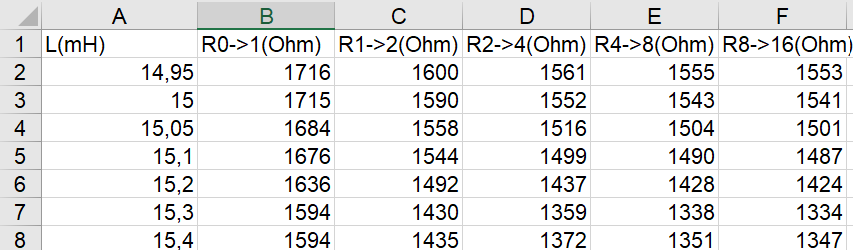
\includegraphics[width=0.6\textwidth]{tableau/Tableau mesures.png}
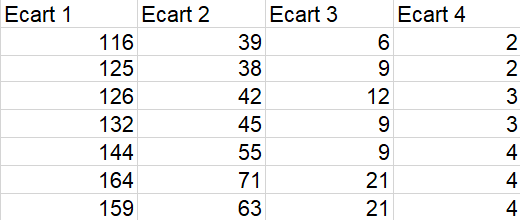
\includegraphics[width=0.4\textwidth]{tableau/tableau ecarts.png}
\caption{Tableaux des valeurs des résistances mesurées et de leurs écarts}
\end{figure}

Sur les mesures, les incertitudes sont plus cohérentes à être prises pour un écart entre deux valeurs de résistances, car bien que les incertitudes sur la valeur absolue de la résistance soit élevée, l'incertitude sur l'écart entre deux valeurs l'est moins car elles ont été effectuées à la suite, donc avec beaucoup de paramètres d'incertitudes en commun (la résistance utilisée était à décades, donc bien que les 1000 $\Omega$ de toutes les mesures soit à $\pm50 ~\Omega $, cette incertitude n'est pas présente pour l'écart entre deux valeurs et n'est donc pas pertinente). On prendra donc 15 $\Omega$, 8 $\Omega$, 3 $\Omega$ et 1,5 $\Omega$ d'incertitudes pour les quatre écarts possibles.\\

Ce qui nous permet de calculer le quotient de deux écarts consécutifs, qui correspondent aux nombres de la suite devant converger vers la constante de Feigenbaum, et leurs incertitudes :

\begin{figure}[H]
\centering
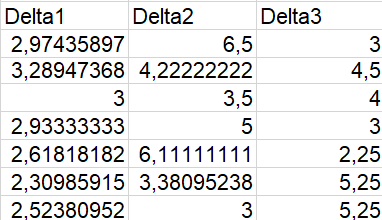
\includegraphics[width=0.4\textwidth]{tableau/tableau delta.png}
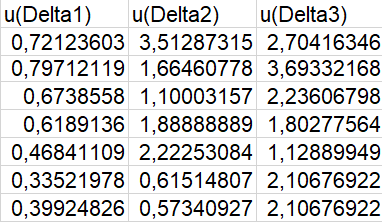
\includegraphics[width=0.38\textwidth]{tableau/tableau incertitudes.png}
\caption{Quotients des écarts et leurs incertitudes}
\end{figure}

Et la moyenne :

\begin{figure}[H]
\centering
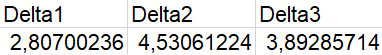
\includegraphics[width=0.5\textwidth]{tableau/tableau moyenne.png}
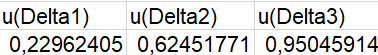
\includegraphics[width=0.5\textwidth]{tableau/tableau incertitudes moyennes.png}
\caption{Moyenne des membres de la suite de Feigenbaum et leurs incertitudes}
\end{figure}

On remarque que les deux dernières valeurs sont de l'ordre de grandeur de la constante de Feigenbaum, ce qui est déjà un bon indicateur du côté chaotique de notre circuit car la convergence vers la constante de Feigenbaum est très rapide \cite[pp.~360--362]{strogatz2018nonlinear}, mais les incertitudes sont trop élevées et il n'y a pas assez de valeurs pour pouvoir calculer une constante de Feigenbaum expérimentale à comparer à la valeur théorique.

\clearpage
\section{Conclusion}

Nous avons donc réussi à créer une diode de Chua grâce à deux amplificateurs opérationnels et six résistances, diode qui a bien la bonne courbe intensité-potentiel. Cette diode nous a permis de créer le circuit de Chua, qui est bien chaotique et permet bien de tracer le << double scroll >> comme prévu par la partie théorique. Ce système nous a ensuite permis d'étudier la transition vers le chaos, donc comment le système passe de point fixe à périodique à chaotique, et de calculer des suites qui selon la partie théorique convergent vers la constante de Feigenbaum. Les valeurs trouvées sont dans le bon ordre de grandeur, mais les incertitudes énormes dues à la sensibilité du système ne permettent pas de vérifier cette convergence, mais nous avons tout de même le bon ordre de grandeur.
\printbibliography
\end{document}
